\section{Logistic Regression}
Classification method

\subsection{Binary Classification}
Decision with 2 possible outcomes (yes, no)

\begin{itemize}
    \item Hail in Lausanne (yes/no)
    \item Master admission (admission / no admission)
    \item Based on different data / entity
\end{itemize}
$y = 1$ implies yes/accepted/admission, $y = 0$ implies no/rejected \\
$P(y = 1, x_1 = 4.5, x_2 = 5, x_3 = 5.5)$\\

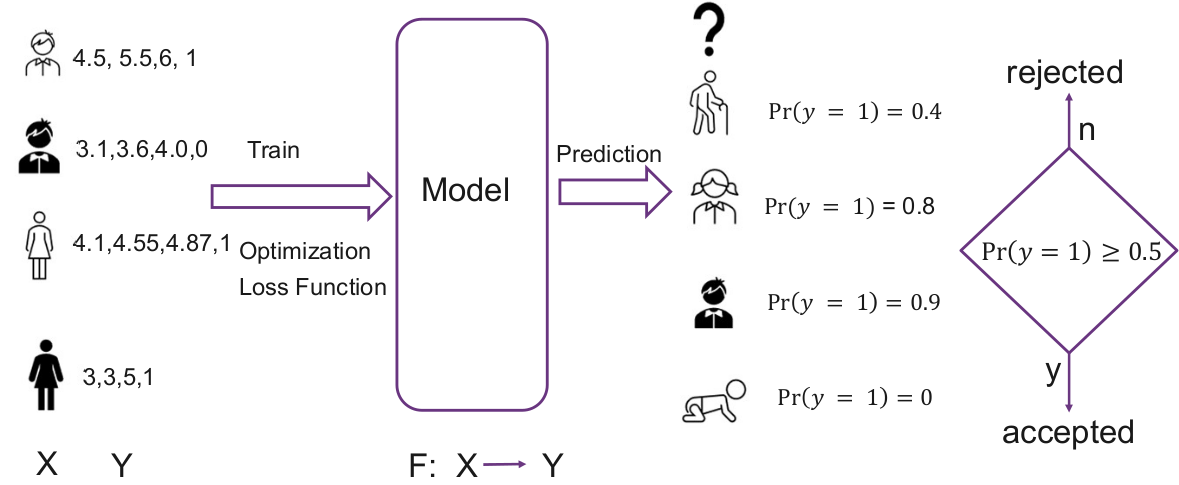
\includegraphics[width=\linewidth]{binary-classification.png}

\subsection{Predicting Probabilities: Logistic Regression}

\textbf{Decision using Linear Regression}
\begin{itemize}
    \item Train the model with gradient descent
    \item \textcolor{red}{Bad Idea!}
    \item Models the response (y) and post process the response (e.g.\ by thresholding) to compute the probability
    \item MSE minimiert den Unterschied von $\hat{y}$ und $y$, was nichts mit der Classification Wahrscheinlichkeit zu tun hat
\end{itemize}
\vspace{10pt}
\textbf{Sigmoid function (the model)}

\begin{itemize}
    \item Values between 0 and 1. $y$ is interpreted as probability
    \item \textcolor{blue}{Function is not parametrized}
    \item Has a single input value
\end{itemize}

\begin{center}
    $sigmoid(y) = \frac{1}{1 + e^{-y}}$
\end{center}
$y$ is

\begin{itemize}
    \item calculated from the input data
    \item a linear combination of the input features, with one feature $ax_i + b$ with D dimensions $y_i=\sum_{d=0}^{d=D}w_d \cdot x_i^d$
    \item e.g. $y = w_1 x_1 + w_2 x_2 + w_3 x_3 + w_4 x_4$
\end{itemize}
\vspace{10pt}
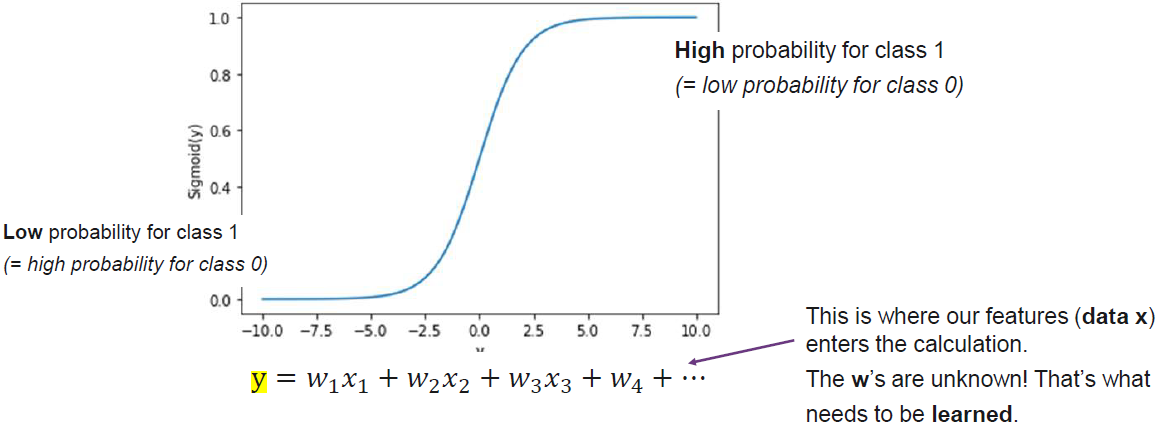
\includegraphics[width=\linewidth]{sigmoid.png} \\

\textbf{Probabilities}
\begin{itemize}
    \item We can write the estimated probability
    \item For a prediction we can write
\end{itemize}
\begin{center}
    $P(x) = \frac{1}{1 + e^{-(W^{T}x)}}$
\end{center}
\vspace{10pt}
\begin{center}
    For example $Pr(y_i = 1 | x_i; w) = \Large \frac {1}{1 + e^{-(w_0 + w_1 \cdot x_{i, 1} + w_2 \cdot x_{i, 2} + w_3 \cdot x_{i, 3})}}$
\end{center}

\subsection{Optimization: Maximum Likelihood Estimation - Loss Function}
\begin{itemize}
    \item \textcolor{blue}{Given all the data points (X,Y) we want to maximize the probability that all the predictions are correct.}
    \item For each of the training data, we want to maximize the likelihood of correct prediction
    \item We can use \textcolor{blue}{Gradient Descent to find optimal $W$}
\end{itemize}
\vspace{10pt}
\begin{center}
    Minimize $cost(W) = E = -\frac{1}{N}\sum_{i=1}^N (y_i \cdot log(p_i)) + (1 - y_i) \cdot log(1 - p_i))$
\end{center}
\vspace{10pt}
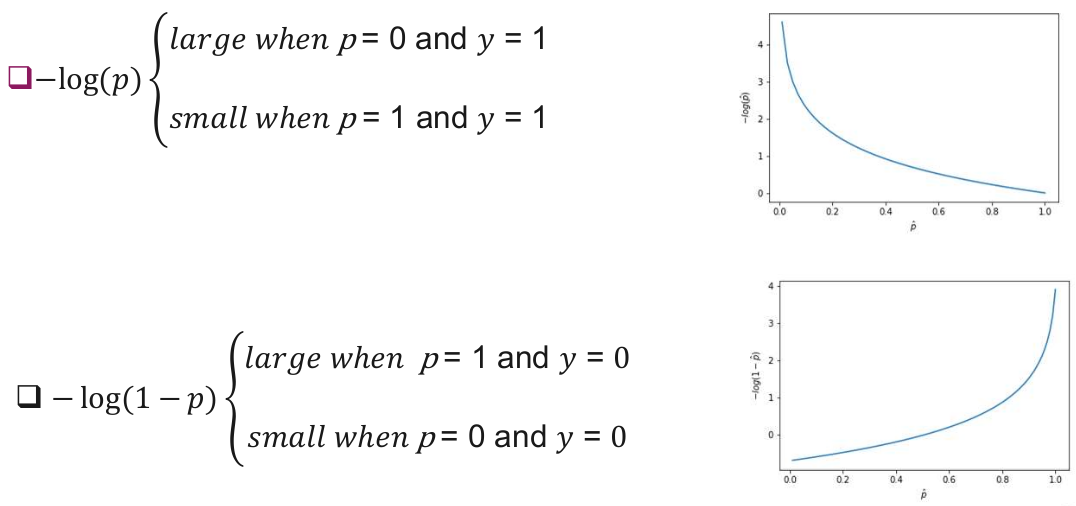
\includegraphics[width=\linewidth]{likelihood-cost.png}

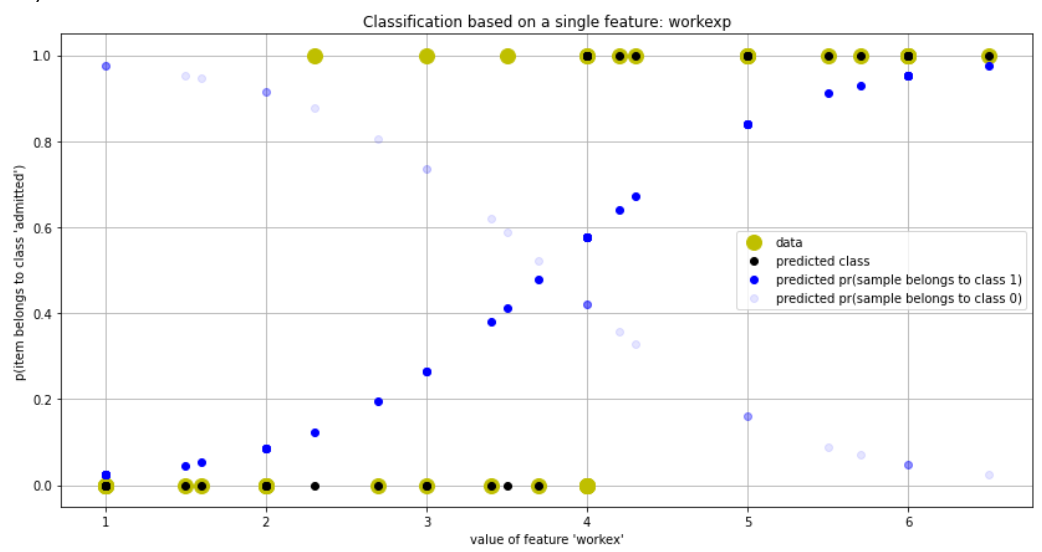
\includegraphics[width=\linewidth]{classification-based-diagram.png}
